\documentclass[journal]{IEEEtran}
% *** GRAPHICS RELATED PACKAGES ***
\usepackage{graphicx}
\usepackage{multirow}
\usepackage{url}

%
\ifCLASSINFOpdf
  % \usepackage[pdftex]{graphicx}
  % declare the path(s) where your graphic files are
  % \graphicspath{{../pdf/}{../jpeg/}}
  % and their extensions so you won't have to specify these with
  % every instance of \includegraphics
  % \DeclareGraphicsExtensions{.pdf,.jpeg,.png}
\else
  % or other class option (dvipsone, dvipdf, if not using dvips). graphicx
  % will default to the driver specified in the system graphics.cfg if no
  % driver is specified.
  % \usepackage[dvips]{graphicx}
  % declare the path(s) where your graphic files are
  % \graphicspath{{../eps/}}
  % and their extensions so you won't have to specify these with
  % every instance of \includegraphics
  % \DeclareGraphicsExtensions{.eps}
\fi
% graphicx was written by David Carlisle and Sebastian Rahtz. It is
% required if you want graphics, photos, etc. graphicx.sty is already
% installed on most LaTeX systems. The latest version and documentation
% can be obtained at: 
% http://www.ctan.org/pkg/graphicx
% Another good source of documentation is "Using Imported Graphics in
% LaTeX2e" by Keith Reckdahl which can be found at:
% http://www.ctan.org/pkg/epslatex
%
% latex, and pdflatex in dvi mode, support graphics in encapsulated
% postscript (.eps) format. pdflatex in pdf mode supports graphics
% in .pdf, .jpeg, .png and .mps (metapost) formats. Users should ensure
% that all non-photo figures use a vector format (.eps, .pdf, .mps) and
% not a bitmapped formats (.jpeg, .png). The IEEE frowns on bitmapped formats
% which can result in "jaggedy"/blurry rendering of lines and letters as
% well as large increases in file sizes.
%
% You can find documentation about the pdfTeX application at:
% http://www.tug.org/applications/pdftex

% *** MATH PACKAGES ***
%
%\usepackage{amsmath}
% A popular package from the American Mathematical Society that provides
% many useful and powerful commands for dealing with mathematics.
%
% Note that the amsmath package sets \interdisplaylinepenalty to 10000
% thus preventing page breaks from occurring within multiline equations. Use:
%\interdisplaylinepenalty=2500
% after loading amsmath to restore such page breaks as IEEEtran.cls normally
% does. amsmath.sty is already installed on most LaTeX systems. The latest
% version and documentation can be obtained at:
% http://www.ctan.org/pkg/amsmath

% *** SPECIALIZED LIST PACKAGES ***
%
%\usepackage{algorithmic}
% algorithmic.sty was written by Peter Williams and Rogerio Brito.
% This package provides an algorithmic environment fo describing algorithms.
% You can use the algorithmic environment in-text or within a figure
% environment to provide for a floating algorithm. Do NOT use the algorithm
% floating environment provided by algorithm.sty (by the same authors) or
% algorithm2e.sty (by Christophe Fiorio) as the IEEE does not use dedicated
% algorithm float types and packages that provide these will not provide
% correct IEEE style captions. The latest version and documentation of
% algorithmic.sty can be obtained at:
% http://www.ctan.org/pkg/algorithms
% Also of interest may be the (relatively newer and more customizable)
% algorithmicx.sty package by Szasz Janos:
% http://www.ctan.org/pkg/algorithmicx

% *** ALIGNMENT PACKAGES ***
%
%\usepackage{array}
% Frank Mittelbach's and David Carlisle's array.sty patches and improves
% the standard LaTeX2e array and tabular environments to provide better
% appearance and additional user controls. As the default LaTeX2e table
% generation code is lacking to the point of almost being broken with
% respect to the quality of the end results, all users are strongly
% advised to use an enhanced (at the very least that provided by array.sty)
% set of table tools. array.sty is already installed on most systems. The
% latest version and documentation can be obtained at:
% http://www.ctan.org/pkg/array

% IEEEtran contains the IEEEeqnarray family of commands that can be used to
% generate multiline equations as well as matrices, tables, etc., of high
% quality.

% *** SUBFIGURE PACKAGES ***
%\ifCLASSOPTIONcompsoc
%  \usepackage[caption=false,font=normalsize,labelfont=sf,textfont=sf]{subfig}
%\else
%  \usepackage[caption=false,font=footnotesize]{subfig}
%\fi
% subfig.sty, written by Steven Douglas Cochran, is the modern replacement
% for subfigure.sty, the latter of which is no longer maintained and is
% incompatible with some LaTeX packages including fixltx2e. However,
% subfig.sty requires and automatically loads Axel Sommerfeldt's caption.sty
% which will override IEEEtran.cls' handling of captions and this will result
% in non-IEEE style figure/table captions. To prevent this problem, be sure
% and invoke subfig.sty's "caption=false" package option (available since
% subfig.sty version 1.3, 2005/06/28) as this is will preserve IEEEtran.cls
% handling of captions.
% Note that the Computer Society format requires a larger sans serif font
% than the serif footnote size font used in traditional IEEE formatting
% and thus the need to invoke different subfig.sty package options depending
% on whether compsoc mode has been enabled.
%
% The latest version and documentation of subfig.sty can be obtained at:
% http://www.ctan.org/pkg/subfig

% *** FLOAT PACKAGES ***
%
%\usepackage{fixltx2e}
% fixltx2e, the successor to the earlier fix2col.sty, was written by
% Frank Mittelbach and David Carlisle. This package corrects a few problems
% in the LaTeX2e kernel, the most notable of which is that in current
% LaTeX2e releases, the ordering of single and double column floats is not
% guaranteed to be preserved. Thus, an unpatched LaTeX2e can allow a
% single column figure to be placed prior to an earlier double column
% figure.
% Be aware that LaTeX2e kernels dated 2015 and later have fixltx2e.sty's
% corrections already built into the system in which case a warning will
% be issued if an attempt is made to load fixltx2e.sty as it is no longer
% needed.
% The latest version and documentation can be found at:
% http://www.ctan.org/pkg/fixltx2e

%\usepackage{stfloats}
% stfloats.sty was written by Sigitas Tolusis. This package gives LaTeX2e
% the ability to do double column floats at the bottom of the page as well
% as the top. (e.g., "\begin{figure*}[!b]" is not normally possible in
% LaTeX2e). It also provides a command:
%\fnbelowfloat
% to enable the placement of footnotes below bottom floats (the standard
% LaTeX2e kernel puts them above bottom floats). This is an invasive package
% which rewrites many portions of the LaTeX2e float routines. It may not work
% with other packages that modify the LaTeX2e float routines. The latest
% version and documentation can be obtained at:
% http://www.ctan.org/pkg/stfloats
% Do not use the stfloats baselinefloat ability as the IEEE does not allow
% \baselineskip to stretch. Authors submitting work to the IEEE should note
% that the IEEE rarely uses double column equations and that authors should try
% to avoid such use. Do not be tempted to use the cuted.sty or midfloat.sty
% packages (also by Sigitas Tolusis) as the IEEE does not format its papers in
% such ways.
% Do not attempt to use stfloats with fixltx2e as they are incompatible.
% Instead, use Morten Hogholm'a dblfloatfix which combines the features
% of both fixltx2e and stfloats:
%
% \usepackage{dblfloatfix}
% The latest version can be found at:
% http://www.ctan.org/pkg/dblfloatfix

%\ifCLASSOPTIONcaptionsoff
%  \usepackage[nomarkers]{endfloat}
% \let\MYoriglatexcaption\caption
% \renewcommand{\caption}[2][\relax]{\MYoriglatexcaption[#2]{#2}}
%\fi
% endfloat.sty was written by James Darrell McCauley, Jeff Goldberg and 
% Axel Sommerfeldt. This package may be useful when used in conjunction with 
% IEEEtran.cls'  captionsoff option. Some IEEE journals/societies require that
% submissions have lists of figures/tables at the end of the paper and that
% figures/tables without any captions are placed on a page by themselves at
% the end of the document. If needed, the draftcls IEEEtran class option or
% \CLASSINPUTbaselinestretch interface can be used to increase the line
% spacing as well. Be sure and use the nomarkers option of endfloat to
% prevent endfloat from "marking" where the figures would have been placed
% in the text. The two hack lines of code above are a slight modification of
% that suggested by in the endfloat docs (section 8.4.1) to ensure that
% the full captions always appear in the list of figures/tables - even if
% the user used the short optional argument of \caption[]{}.
% IEEE papers do not typically make use of \caption[]'s optional argument,
% so this should not be an issue. A similar trick can be used to disable
% captions of packages such as subfig.sty that lack options to turn off
% the subcaptions:
% For subfig.sty:
% \let\MYorigsubfloat\subfloat
% \renewcommand{\subfloat}[2][\relax]{\MYorigsubfloat[]{#2}}
% However, the above trick will not work if both optional arguments of
% the \subfloat command are used. Furthermore, there needs to be a
% description of each subfigure *somewhere* and endfloat does not add
% subfigure captions to its list of figures. Thus, the best approach is to
% avoid the use of subfigure captions (many IEEE journals avoid them anyway)
% and instead reference/explain all the subfigures within the main caption.
% The latest version of endfloat.sty and its documentation can obtained at:
% http://www.ctan.org/pkg/endfloat
%
% The IEEEtran \ifCLASSOPTIONcaptionsoff conditional can also be used
% later in the document, say, to conditionally put the References on a 
% page by themselves.

% *** PDF, URL AND HYPERLINK PACKAGES ***
%
%\usepackage{url}
% url.sty was written by Donald Arseneau. It provides better support for
% handling and breaking URLs. url.sty is already installed on most LaTeX
% systems. The latest version and documentation can be obtained at:
% http://www.ctan.org/pkg/url
% Basically, \url{my_url_here}.

% *** Do not adjust lengths that control margins, column widths, etc. ***
% *** Do not use packages that alter fonts (such as pslatex).         ***
% There should be no need to do such things with IEEEtran.cls V1.6 and later.
% (Unless specifically asked to do so by the journal or conference you plan
% to submit to, of course. )

% correct bad hyphenation here
\hyphenation{op-tical net-works semi-conduc-tor}

\begin{document}
%
% paper title
% Titles are generally capitalized except for words such as a, an, and, as,
% at, but, by, for, in, nor, of, on, or, the, to and up, which are usually
% not capitalized unless they are the first or last word of the title.
% Linebreaks \\ can be used within to get better formatting as desired.
% Do not put math or special symbols in the title.
\title{Diabetes Prediction in Arizona Pima Women
 
Using Random Forest Classifier}
%
%
% author names and IEEE memberships
% note positions of commas and nonbreaking spaces ( ~ ) LaTeX will not break
% a structure at a ~ so this keeps an author's name from being broken across
% two lines.
% use \thanks{} to gain access to the first footnote area
% a separate \thanks must be used for each paragraph as LaTeX2e's \thanks
% was not built to handle multiple paragraphs
%

\author{Annie~Tran,~
        Ivan~Cvjetinovic,~
        Nikko~Sanchez,~
        and~Wanzhu~Zheng}% <-this % stops a space

% The paper headers
\markboth{ECS 171, Machine Learning}%
{Shell \MakeLowercase{\textit{et al.}}: Diabetes Classification in Pima Women}

\maketitle

\begin{abstract}
Early diagnosis of type 2 diabetes (T2D) remains a hot topic in research. Unlike type 1 diabetes, T2D is largely preventable; for this reason, prediction is vital for early and effective prevention. Several risk factors have been identified, including age, body weight, abdominal fat storage, physical inactivity, genetic predisposition, number of pregnancies, and more. In this paper, our focus is on a high-risk population—the Pima Indians of Arizona—and eight different risk factors that were studied in a 1965 longitudinal study: number of pregnancies, glucose concentration, blood pressure, triceps skin fold thickness, insulin level, body mass index (BMI), genetic risk factor, and age. We propose a Random Forest Classifier model that predicts the presence of T2D in a patient given their medical data on the most informational risk factors, which we identify through machine learning analytics. Our model demonstrates an accuracy of about 77\%, which is decent but leaves room for considerable improvement.

\textit{Keywords: Diabetes mellitus; type 2 diabetes; Pima Indians; diagnosis; classification; prediction; machine learning; healthcare}
\end{abstract}

\IEEEpeerreviewmaketitle

\section{Introduction}
\IEEEPARstart{T}{ype} 2 diabetes (T2D), otherwise known as diabetes mellitus, is a chronic medical condition in which the body is either resistant to insulin or unable to produce a sufficient amount of insulin. Although T2D has no cure, its onset can be prevented through the implementation of healthy lifestyle changes, such as adopting a healthier diet and exercising more frequently (Mayo Clinic 2023).

One population that has been disproportionately affected by T2D is the Pima Tribe of Arizona. The arrival of European colonizers in Arizona upturned the Pimas' active lifestyle (Schulz and Chaudhari 2015). Traditionally, the Pimas of Arizona relied on a complex canal system to irrigate their farms. However, as European colonizers settled on the land, the waterway was diverted and food scarcity - often leading to famine - became a rampant issue (Schulz and Chaudhari 2015). Around the same time as this drastic change to a sedentary and food-insecure lifestyle, the presence of diabetes among the Arizona Pima population rose, and prevalence reached a high surpassing all past records of T2D, according to a study from 1965 (Schulz and Chaudhari 2015).

Certain risk factors may increase the chance of developing T2D, including older age, high body weight, high fat storage in the abdomen, minimal physical activity, genetic family history, and gestational diabetes (Mayo Clinic 2023). In a longitudinal study on Pima women in Arizona, starting in 1965 and lasting more than 10 years, researchers focused on eight potential predictors of T2D: number of pregnancies, glucose concentration from Oral Glucose Tolerance Test (OGTT), blood pressure (mmHg), triceps skin fold thickness (mm), insulin level ($\mu$U/ml), body mass index (BMI) score, Diabetes Pedigree Function, and age in years (Smith et al. 1988).

Given that accurate prediction precedes effective prevention, we will develop an optimal prediction model to determine whether a patient may have T2D based on the input of medical information for the most relevant predictors. Through this endeavor, we also hope to discover broader trends that can be applied to improve future T2D diagnostics and can provide us with a clearer understanding of the relationship between various medical features and T2D development, ultimately having important applications in the wider scope of improving healthcare coverage for a historically marginalized and undeserved population.

This paper first reviews machine learning studies previously done on the same Pima dataset, then goes on to describe the dataset, including its features, target variable, and demographic of focus. Then it describes the workflow of our project, starting with pre-processing and exploratory data analysis, up to model development and evaluation. Finally, this paper discusses the limitations of our final model as well as the Pima dataset itself, with suggestions for improvement in follow-up studies.

% You must have at least 2 lines in the paragraph with the drop letter

\section{Literature Review}
In our review of relevant and previous works, we sought to gain more information about the demographic we chose to study—the Pima Indian women of Arizona—as well as the machine learning algorithms past researchers have applied on our dataset of interest.\\

Schulz and Chaudhari (2015) explore the "thrifty gene" hypothesis, which posits that genes favoring fat storage were historically advantageous during periods of famine but have become a risk factor for obesity and type II diabetes in modern times due to increased food availability. The Pima Indians in Arizona, who are the population of interest in this study, exemplify this hypothesis. Their transition to a modern lifestyle has resulted in heightened rates of both obesity and type II diabetes.

In contrast, the Pima Indians in Mexico, who share the same genetic background as their counterparts in Arizona but lead more active lifestyles with less abundant food supplies, exhibit lower levels of insulin resistance, a risk factor for type II diabetes. This suggests that environmental factors significantly influence the prevention of type II diabetes among individuals genetically predisposed to the condition. The study highlights that environmental factors are the primary drivers for the development of type II diabetes, as evidenced by the increased prevalence among Pima women transitioning to modern lifestyles. \\

In a machine learning study, Smith et al. (1988) focus on utilizing the ADAP learning algorithm, a neural network, to predict the onset of diabetes mellitus. Like other neural networks, ADAP makes internal corrections as it proceeds with its predictions on the training dataset. In the conclusion of this paper, ADAP proves to demonstrate an impressive discriminate capacity, producing a ROC curve located quite close to the upper left corner of the graph boundary. 

The dataset used in Smith et al.'s study consists exclusively of female Pima patients aged 21 and above. One of the critical features examined is the Glucose Tolerance Test (GTT), which serves as an indicator of the likelihood of developing T2D; lower GTT values correspond to a decreased likelihood of developing the condition. Another feature, the Diabetes Pedigree Function, is a mathematical method for calculating genetic propensity for type II diabetes based on the occurrence of the disease among family members.

The researchers divide the dataset into 75\% training data (comprising 768 subjects or examinations) and 25\% testing data (comprising 192 examinations). Given the comprehensive feature engineering already performed on this dataset by experts in T2D research within Pima populations, the researchers opt to retain these selections without making any additional modifications.\\

A later study, conducted by researchers Aishwarya Mujumdar and Dr. Vaidehi V in 2019, compares the performance of a variety of machine learning algorithms, including Logistic Regression, Gradient Boost Classifier, LDA, AdaBoost Classifier, Extra Trees Classifier, Gaussian NB, Bagging, Random Forest, Decision Tree, Perceptron, SVC, and KNN. The application of these algorithms to the Pima dataset we use in our own study does not stand out; the accuracies of predictions lie in the range of high 60s to high 70s. However, when applied to the researchers' new diabetes dataset, the accuracies skyrocket, with the highest being 96\% with a Logistic Regression model. In this way, the researchers demonstrate that model performance can be drastically improved with additional training on a better dataset. The model accuracies see further improvement with pipelining, which yields AdaBoost Classifier as the best model, boasting an accuracy of 98.8\%.\\

In a more recent study we looked at, researcher Omer Faruk Akmese (2022) explores T2D diagnostics, applying various machine learning techniques to the same dataset as the previous studies as well as our own. Akmese addresses the issue of zero values for Glucose, Blood Pressure, Skin Thickness, Insulin, and BMI by replacing them with mean values. Visualization of the data yields findings consistent with those presented in the following section of our paper. To manage outliers and missing values, Akmese similarly employs a strategy of replacing them with mean values, ensuring the dataset's integrity for subsequent machine learning applications.\\

The most recent paper we reviewed, by Chang et al. (2022) examines the relevance of artificial intelligence and machine learning in healthcare, and compared three different supervised machine learning algorithms applied to the Pima dataset: Naive Bayes classifier, Random Forest classifier, and J48 decision tree. 

First, AI and machine learning play an important role in healthcare by providing a preliminary diagnosis of disease, such as T2D in our case, which can then be confirmed by the doctor. Such predictive tools save time and resources for healthcare providers, while also expediting the process of determining an official diagnosis for a patient. The importance of AI and machine learning becomes increasingly evident when one considers the case of complex conditions, such as T2D, where multiple factors come into play and some patients may not exhibit typical symptoms early on. The predictive prowess of these computational tools helps to identify underlying patterns in a patient's medical history and status that a human may not be able to early on, at least not without expending a significant amount of resources on an individual patient—an unfeasible feat, given that healthcare providers must already stretch themselves thin in an effort to serve a sizeable population of patients. 

Secondly, researchers found that Random Forest yielded the best performance with the full Pima dataset, compared to Naive Bayes and J48. However, Naive Bayes had the best performance when feature selection was applied to the dataset, reducing the amount of features to 3 in one experiment and 5 in another.
\\

\section{Data Description}
The dataset used for the Arizona Pima Women study on diabetes prediction consists of medical records of 768 patients, all of whom are female and 21 years of age or older. These women belong to Pima Indian heritage, a demographic known to have a higher risk of diabetes. The dataset includes eight attributes that are relevant for predicting diabetes:

\begin{itemize}
    \item \textbf{Number of pregnancies:} The total number of times a patient has been pregnant
    \item \textbf{Glucose Concentration:} Measured from the Oral Glucose Tolerance Test (OGTT) in $\frac{mg}{dL}$
    \item \textbf{Blood Pressure:} Diastolic blood pressure measured in mmHg
    \item \textbf{Triceps Skin Fold Thickness:} Measured in millimeters.
    \item \textbf{Insulin Level:} Measured in $\frac{\mu u}{mL}$ 
    \item \textbf{Body Mass Index (BMI):}  Calculated as weight in kg divided by height in meters squared
    \item \textbf{Diabetes Pedigree Function:} A function that scores likelihood of diabetes based on family history
    \item \textbf{Age:} The age of the patient in years.
\end{itemize}

The presence of non-usable zero values in the attributes for triceps skin fold thickness and insulin levels presents a challenge for the analysis. These zero values likely represent missing data rather than true zero measurements, which requires careful handling during the data pre-processing phase to ensure the accuracy and reliability of the predictive models.

\section{Exploratory Data Analysis}
The initial examination of our dataset revealed no identifiable null values, allowing us to proceed directly to data visualization. We generated histograms for all features in the dataset, which revealed that most of the data distributions were heavily skewed prior to imputation. Note that the features: Glucose, Blood Pressure, Skin Thickness, Insulin, and BMI have high values of zeros. Although these values are not null, they are considered to be invalid because a zero value cannot exist for these features. Therefore, we proceed with imputations to account for this inaccuracy.
\begin{center}
    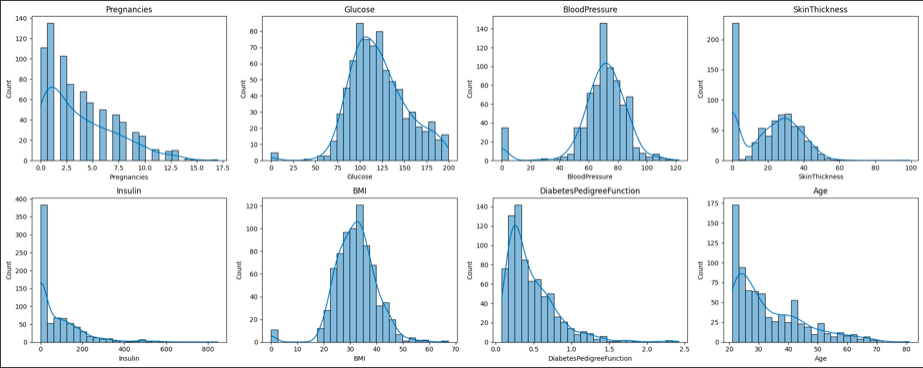
\includegraphics[width=8cm]{DATA-VIZ.png}
\end{center}
\begin{center}
    \textbf{Numerical Benchmark Values for Dataset}
\end{center}
\begin{tabular}{|c|c|c|c|}
     \hline
      & Mean & Median & Standard Deviation \\
     \hline
     Pregnancies & 3.845 & 3.0 & 3.369 \\
     \hline
     Glucose & 120.894 & 117.0 & 31.972 \\
     \hline
     Blood Pressure & 69.105 & 72.0 & 19.355 \\
     \hline
     Skin Thickness & 20.536 & 23.0 & 15.952 \\
     \hline
     Insulin & 79.799 & 30.5 & 115.244 \\
     \hline
     BMI & 31.992 & 32.0 & 7.884 \\
     \hline
     DPF & 0.471 & 0.372 & 0.331 \\
     \hline
     Age & 33.240 & 29.0 & 11.760 \\
     \hline
\end{tabular} \\

To further understand the relationships between features, we visualized feature correlations using a coefficient matrix and multiple scatterplots. These visualizations indicated minimal correlation among the features. 
\begin{center}
    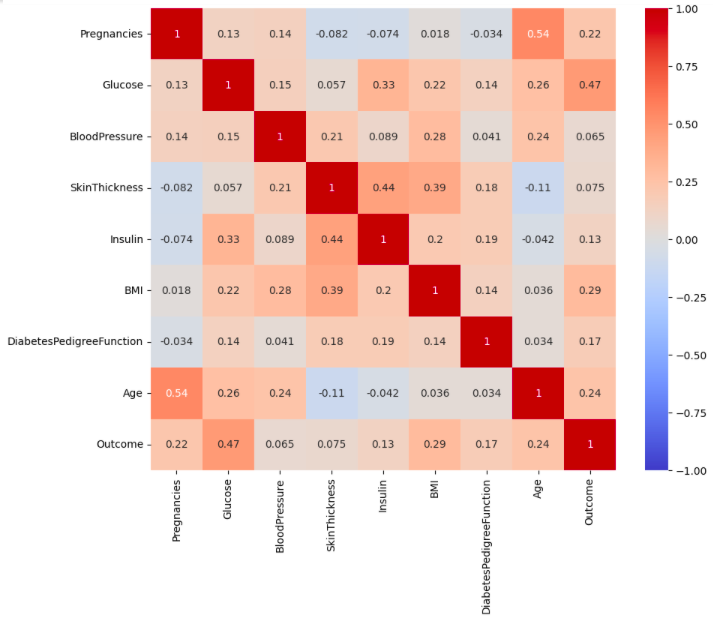
\includegraphics[width=8cm]{DATA-CONF.png}
\end{center}
\begin{center}
    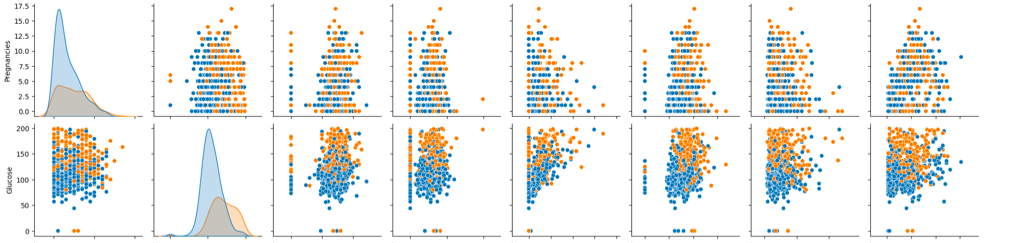
\includegraphics[width=8cm]{scatter1.png}
    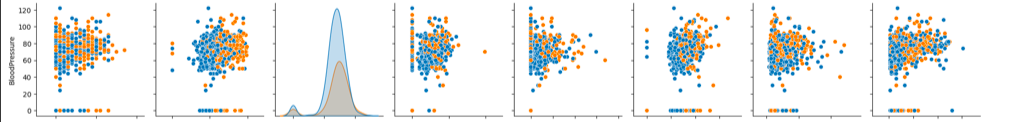
\includegraphics[width=8cm]{scatter2.png}
    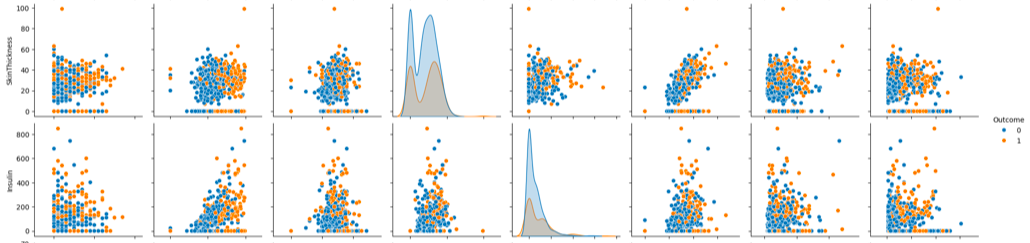
\includegraphics[width=8cm]{scatter3.png}
    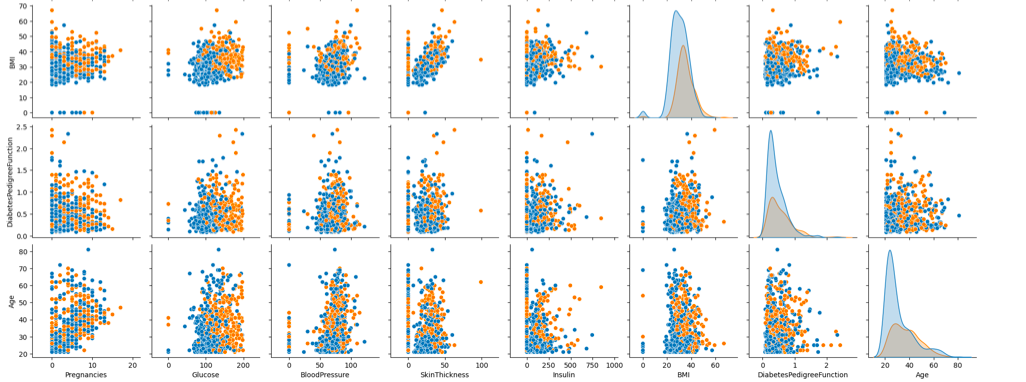
\includegraphics[width=8cm]{scatter4.png}
\end{center}

Despite the imputation performed on our dataset, the presence of outliers remains a concern. Outliers were identified through statistical analysis, specifically using Interquartile Range (IQR) calculations, and machine learning algorithms such as one-class Support Vector Machine (SVM) and Isolation Forest.  \\

\resizebox{0.45\textwidth}{!}{%
\begin{tabular}{ |p{2cm}||p{2cm}|p{2cm}|p{2cm}|  }
 \hline
 \multicolumn{4}{|c|}{Outlier Calculations} \\
 \hline
 \footnotesize Feature & \footnotesize IQR & \footnotesize SVM & \footnotesize Isolation Forest\\
 \hline
 \footnotesize Pregranancies  & 4  & 378  & 387\\
 \footnotesize Gludose        & 5  & 387  & 210\\
 \footnotesize Blood Pressure & 45 & 358  & 144\\
 \footnotesize Skin Thickness & 1  & 222  & 200\\
 \footnotesize Insulin        & 34 & 593  & 123\\
 \footnotesize BMI            & 19 & 396  & 121\\
 \footnotesize DPF            & 29 & 381  & 130\\
 \footnotesize Age            & 9  & 399  & 336\\
 \hline
\end{tabular}}
\\

After numerically analyzing for outliers, we visually represent them with a boxplot.

\begin{center}
    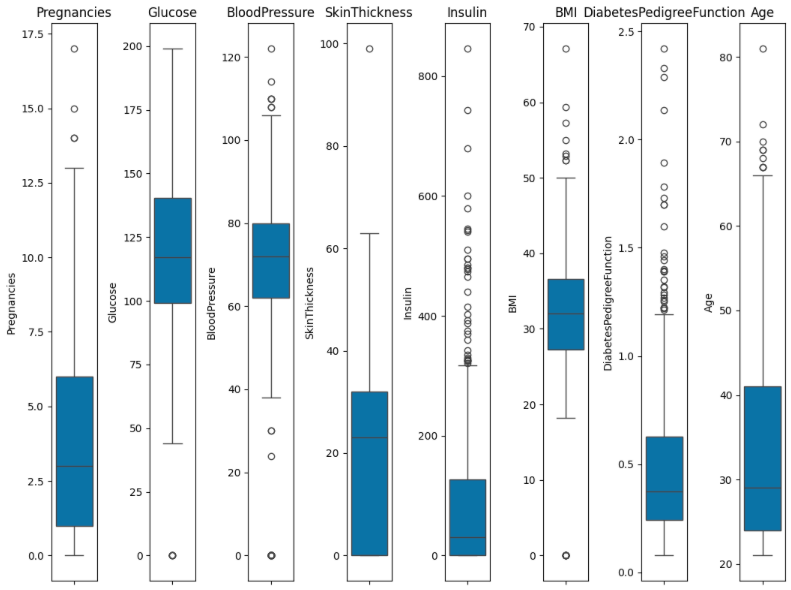
\includegraphics[width=8cm]{BOX.png}
\end{center}

\section{Data Preprocessing}

After analyzing the dataset, our team found a significant number of invalid attribute values. Model development requires the dataset to be clean and statistically sound. We explored some data cleaning and manipulation techniques on the dataset so that it would be ready for model training and testing. Our team identified two options for invalid data: dataset trimming or imputation. Dataset trimming involves invalidating inputs containing at least one invalid attribute or utilizing a random sample from the dataset. We explored two possibilities for feature imputation: the naive imputation approach or running the feature on a K-Nearest Neighbors (KNN) model.


\subsection{Dataset Trimming: Deleting All Invalid Input Values}

The simplest option for dealing with invalid attributes without value manipulation is to remove their associated input data from the sample dataset. After removing all input values with invalid attributes, we found that the size of our dataset significantly reduced from 768 to 392. Since we wanted a more robust sample size for model development, we decided not to utilize this dataset.

\subsection{Dataset Trimming: Random Sampling Without Imputation}

Random Sampling is a technique where random input values are extracted from the dataset and used as a sample. Our team performed 50 random selections on 450 samples from the original dataset. To analyze the technique, we compared the percentage of invalid values for each attribute -- otherwise known as sparsity -- from the original and randomly sampled datasets. After processing the random samples, we found that the random samples either retained or had a larger proportion of invalid data than the original dataset (see tables).

\begin{center}
    \textbf{Sparsity of Original Dataset}
    \begin{tabular}{|c|c|}
        \hline
        Attribute & Sparsity (\%) \\
        \hline
        Glucose & 0.521 \\
        \hline
        Blood Pressure & 2.734 \\
        \hline
        Skin Thickness & 17.708 \\
        \hline
        Insulin & 28.516 \\
        \hline
        BMI & 1.041 \\
        \hline
    \end{tabular}
\end{center}

\begin{center}
    \textbf{Mean and Median Sparsity of Sample Datasets}
    \begin{tabular}{|c|c|c|}
        \hline
        & Mean Sparsity (\%) & Median Sparsity (\%) \\
        \hline
        Glucose & 0.609 & 0.667 \\
        \hline
        Blood Pressure & 4.560 & 4.444 \\
        \hline
        Skin Thickness & 29.387 & 29.333 \\
        \hline
        Insulin & 48.458 & 48.333 \\
        \hline
        BMI & 1.436 & 1.333 \\
        \hline
    \end{tabular} \\
\end{center}

\subsection{Imputation: Naive Method}

The naive imputation method involves overwriting invalid values for attributes with either the mean or median of the valid values. The choice of what statistical value to use for an attribute’s imputation depends on the distribution. We decided to utilize the mean value for normally distributed attributes and the median value for features with a skewed distribution; this decision was made on the basis that the median value does not hold statistical bias and, as a result, overwritten invalid values should not significantly affect the shape of the skew.

It is important to note that naive imputation is discouraged since it heavily implies that the actual distribution of an attribute has the same shape as the distribution of valid values; because of this, we only used the naive approach on features that have an insignificant number of invalid data so that we can retain the same sample size as the original dataset (Dettori, Norvell, and Chapman 2018).

Ultimately, our team decided to utilize the KNN approach for imputation because it would retain the dataset size while estimating the attribute so that invalid values would be statistically sound (IBM n.d.). Two KNN models – one for ‘Skin Thickness’ and one for ‘Insulin Levels’ – were trained and tested on the other attributes modified via the naive method (this excludes ‘Skin Thickness,’ ‘Insulin Levels,’ and ‘Outcome’).

\subsection{Imputation: Results From Combining Naive and KNN Methods}

We analyzed the attribute distributions from imputation with the distributions after simply removing invalid data, and we noticed that both distributions are fairly similar. One notable advantage of the imputed dataset is that it maintains a large sample size, which means that the developed model will have a more robust dataset to train and test on.

\begin{figure}
    \centering
    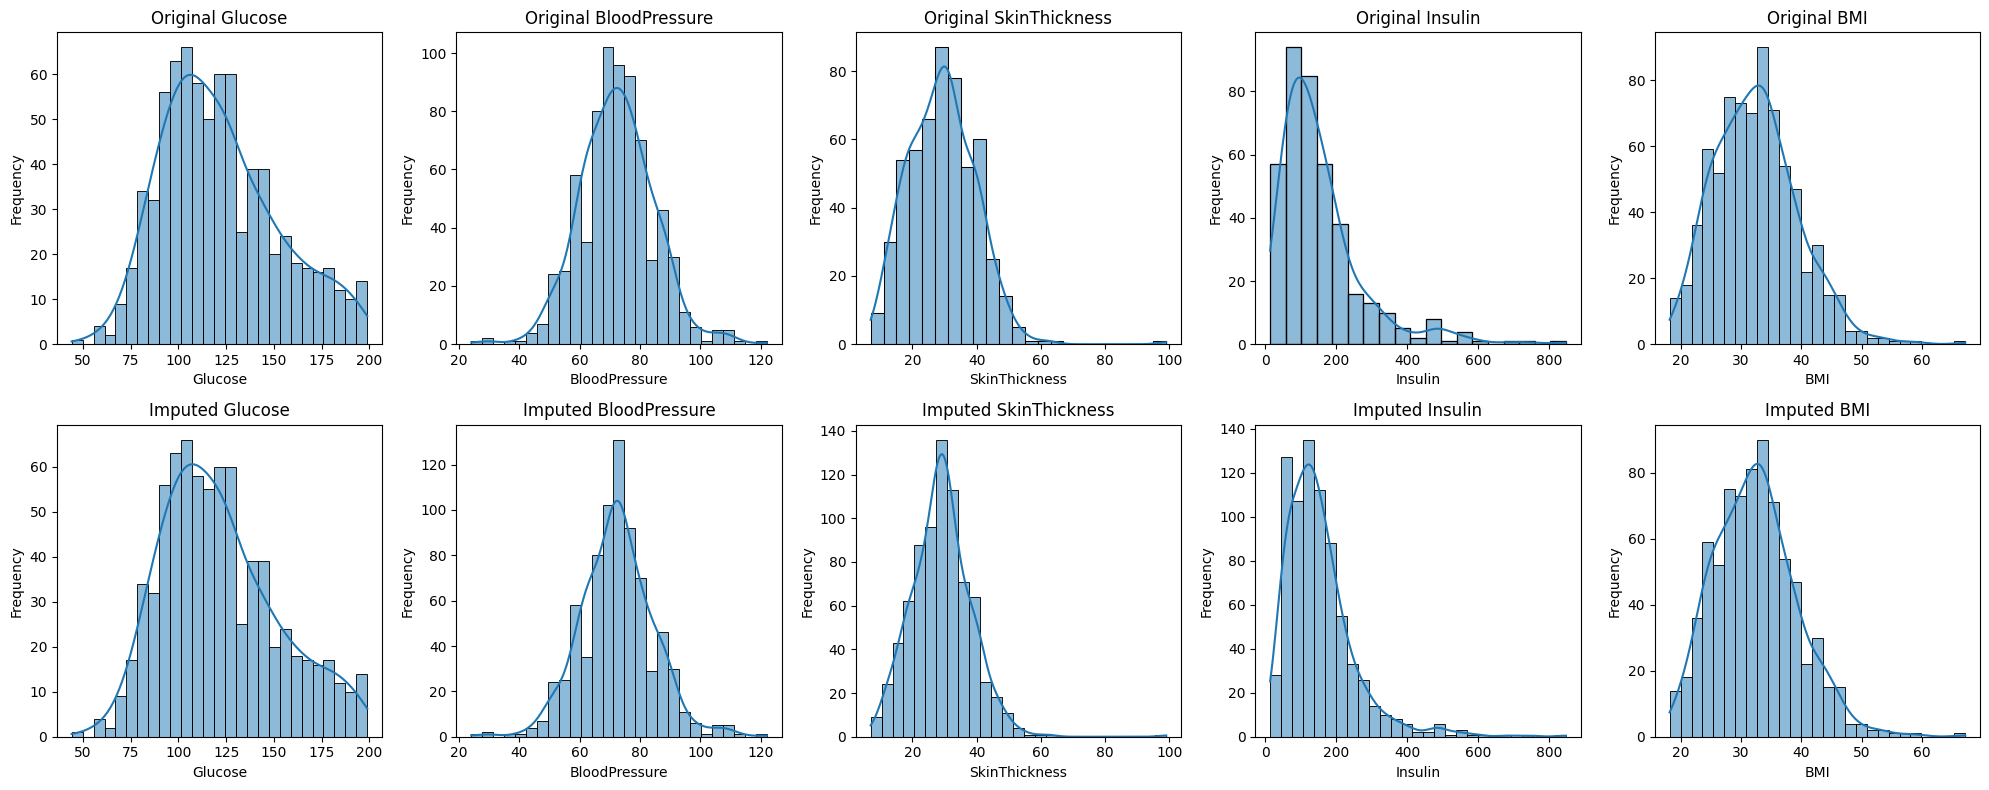
\includegraphics[width=1\linewidth]{original_vs_imputed_dist_shape.png}
    \caption{Comparison Between Original and Imputed Attribute Data Distributions (original on top and imputed on bottom)}
    \label{fig:enter-label}
\end{figure}

The x-axis measures the contribution values, ranging from 0.00 to 0.25. One of the most notable observations is that Glucose has the highest contribution in both original and imputed datasets, with a significant increase after imputation. This means that Glucose levels are a core contributor to whether or not a person has T2D. Other features like Age, BMI, and Insulin also show substantial changes in their contributions following imputation. Showing an increase after imputation suggests that these features have a stronger impact on the model. In contrast, features such as DiabetesPedigreeFunction and BloodPressure display a decrease in their contributions post-imputation. This means that these features are not as statistically significant compared to others. Therefore, less weight should be put on them in our model. Overall, the chart indicates that data imputation gives us a more accurate representation of attribute significance.

\section{Feature Selection}

\subsection{Principal Component Analysis}
Principal Component Analysis (PCA) is a technique commonly employed in feature selection and dimensionality reduction in data analysis. By transforming the original features into a new set of uncorrelated variables, or \textit{principal components}, PCA decreases the complexity of data while retaining the most significant trends.

Prior to applying PCA, we standardized the data using scikit's StandardScaler class. We then applied PCA projection to a 2D space. From here, we compared variance ratios between different subsets of the data, including the entire dataset, the dataset minus "SkinThickness," the dataset minus "Insulin," and the dataset minus both "SkinThickness" and "Insulin."

\emph{Mathematical Reasoning and Proof}
PCA primarily serves as a dimensionality reduction technique, effectively reducing the number of features in a dataset while retaining the most crucial information. This is especially beneficial for high-dimensional data, where many features may be redundant or irrelevant. PCA also facilitates data visualization by reducing complex datasets to two or three dimensions, making it easier to identify patterns, clusters, or outliers. Additionally, PCA aids in noise reduction by discarding less significant components that might represent noise rather than useful signals.

Feature extraction is another advantage of PCA, as it creates new features (principal components) that are linear combinations of the original features, often leading to improved model performance. By reducing the number of features, PCA enhances computational efficiency and reduces memory usage, which is particularly advantageous for large datasets or complex models. It also mitigates multicollinearity by transforming correlated features into a set of uncorrelated components, which can improve the performance of machine learning algorithms.

To find the principal components, PCA performs an eigenvalue decomposition of the covariance matrix. This decomposition results in eigenvectors and corresponding eigenvalues. The eigenvectors represent the directions in which the data varies the most, while the eigenvalues indicate the magnitude of this variance. The principal components are the eigenvectors associated with the largest eigenvalues, forming a new basis for the data.

For dimensionality reduction, one selects the top $k$ eigenvectors that correspond to the largest eigenvalues. These eigenvectors are then used to project the original data onto a new $k$-dimensional subspace, resulting in a transformed data matrix. This projection retains the maximum variance within the reduced dimensionality, summarizing the essential features of the dataset.

The mathematical steps of PCA ensure that the transformed data has zero mean and captures the directions of maximum variance. By centering the data, computing the covariance matrix, performing eigenvalue decomposition, selecting the top eigenvectors, and projecting the data onto this new basis, PCA effectively reduces dimensionality while preserving the most significant patterns in the data. This makes PCA a powerful tool for simplifying complex datasets and enhancing computational efficiency in machine learning tasks.

Ultimately, in our application of PCA to the Pima dataset, we did not find differences in the variance ratios between the subsets of the data that were significant enough to justify removing certain features. Thus, we moved onto Random Forest for our feature selection task.

\subsection{Random Forest Feature Selection}
Random forests are commonly used to determine feature importance due to several key advantages. As an ensemble method, random forests combine multiple decision trees to enhance predictive performance and reduce over-fitting. This approach yields more robust estimates of feature importance by averaging the results from many trees. During the training process, random forests inherently evaluate feature importance by calculating the decrease in impurity (such as Gini impurity or entropy) each time a feature is used to split a node. Features that lead to significant decreases in impurity are deemed more important. Based on the produced plot, we see that Glucose is the biggest feature contributor (Fig. 2).

\begin{figure}
    \centering
    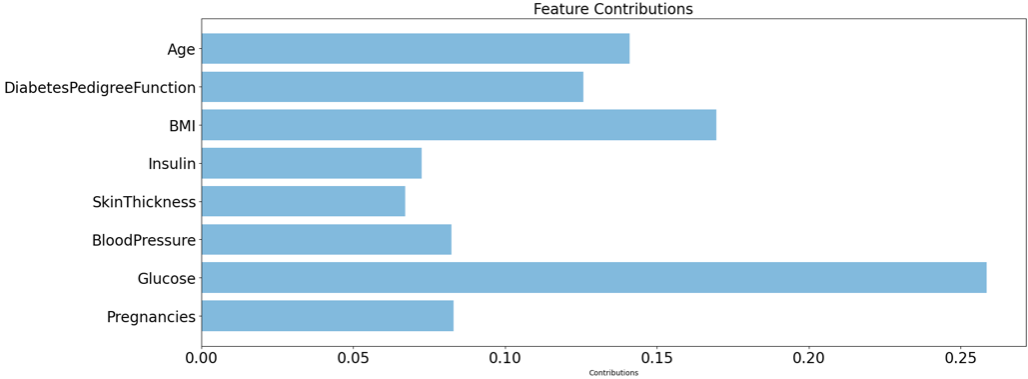
\includegraphics[width=8cm]{FEATURE.png}
    \caption{The ROC curve shows the performance of the model across different classification thresholds}
    \label{fig:enter-label}
\end{figure}

\begin{figure}
    \centering
    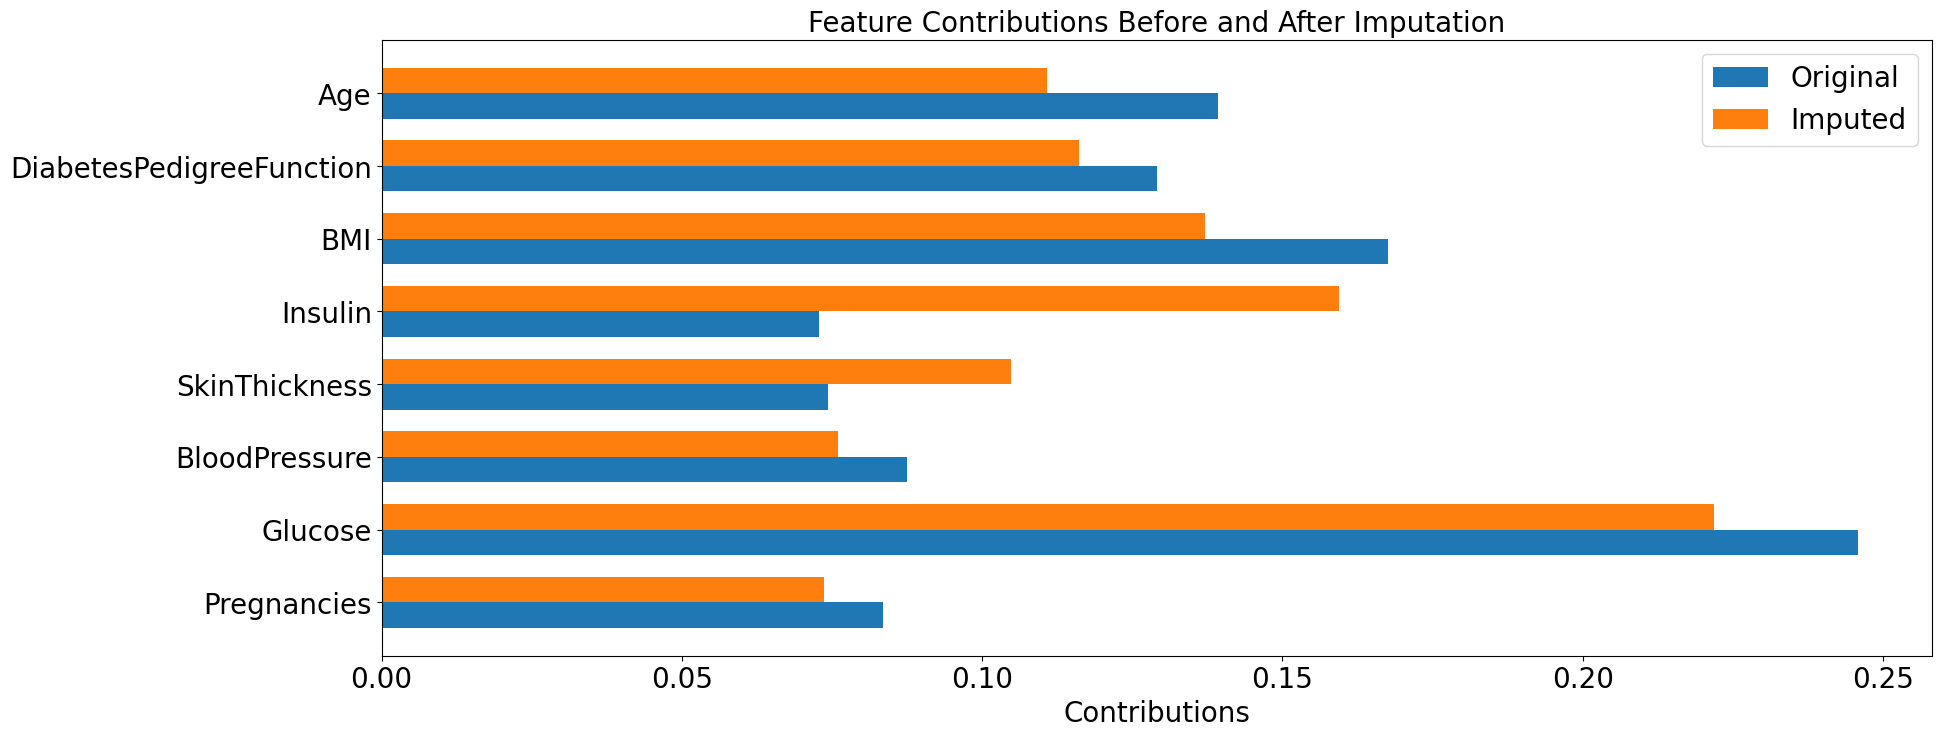
\includegraphics[width=1\linewidth]{pre_and_post-bjffoihewqorjewifewqojfoeqwiiqewjofhiwhfuewoq.png}
    \caption{Random Forest Classification on pre-imputed and post-imputed data}
    \label{fig:enter-label}
\end{figure}

\section{Model Development}

\subsection{Dataset Splitting}
Having performed \textit{Feature Selection} during our pre-processing, we now rely on this background knowledge in order to locate an optimal training dataset.
\begin{center}
NOTE: Reference Section VI for Feature Selection $^{(a)}$
\end{center}
We proposed and tested model variations on both the Original and Imputed Datasets, proceeding to divide the Imputed Dataset into several partitions, removing the following features in relation to their corresponding feature contribution scores:

\begin{itemize}
\item Pregnancies - lowest score post-imputation
\item Skin Thickness and Insulin - lowest scores pre-imputation; held a 30\% and 49\% data sparsity, respectively 
\end{itemize}

We also decided to consider the effects of applying a Bagged Decision Tree on our dataset in contrast to Random Forest. This reason stemmed from the idea that Random Forest may have supplied an unnecessary added degree of stochasticity which did not suit this specific diabetes classification problem. 

A modification we made towards validating the success of each model was done via cross validation. Using the inherent trait of the k-folds algorithm, where a dataset is split apart into multiple folds, we trained and evaluated the model on several different dataset configurations, aggregating accuracies into a finalized mean score expressing the proficiency of each model. 

Introducing this element of randomness ensured both high and low performing occurrences were taken into account towards model evaluation. This randomness helps grade the model on how it would perform on varying subsets of brand new data. Skipping this step would provide a lackluster analysis wherein only a single configuration of unknown data would be tested, producing biased results. 

\section{Results}

\begin{figure}
\centering
    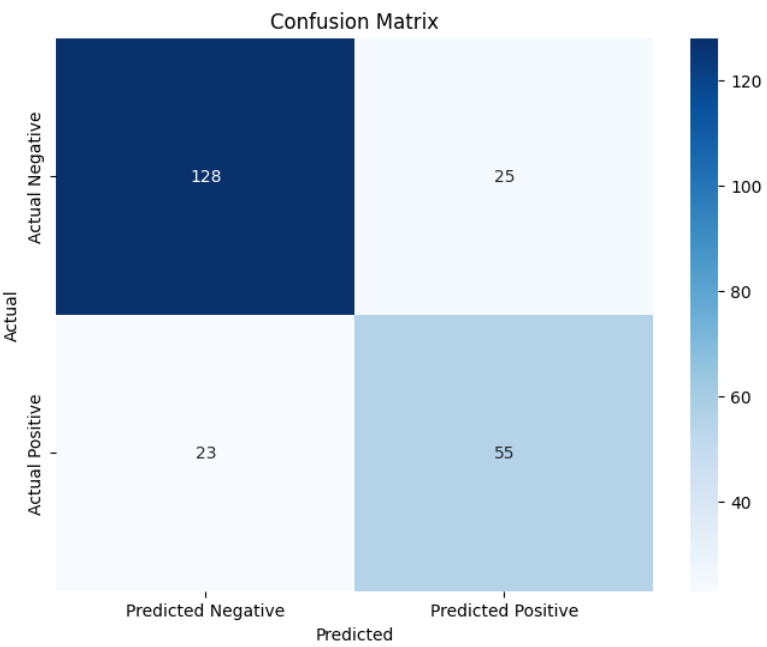
\includegraphics[width=8cm]{CONF.png}
    \caption{This confusion matrix provides a detailed breakdown of the model's predictions versus the actual outcomes}
    \label{fig:enter-label}
\end{figure}

\begin{figure}
    \centering
    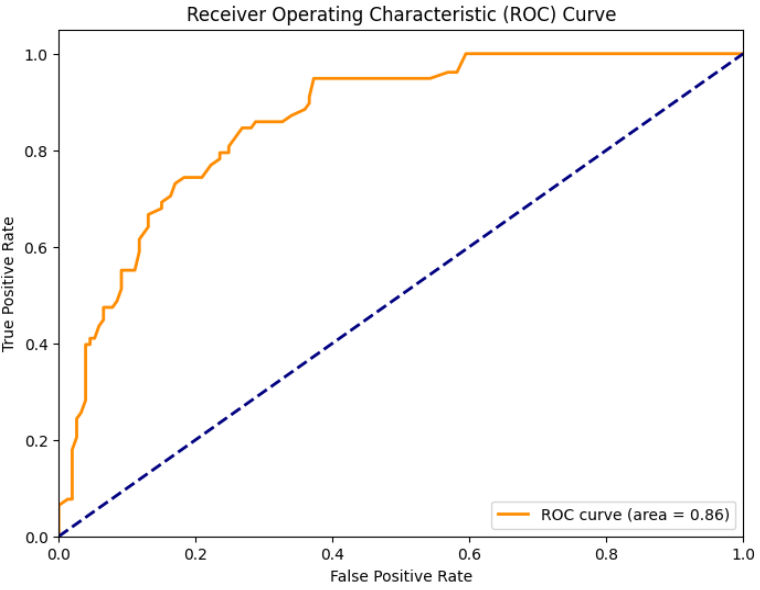
\includegraphics[width=8cm]{ROC.png}
    \caption{The ROC curve shows the performance of the model across different classification thresholds}
    \label{fig:enter-label}
\end{figure}

\normalsize
\subsection{Index Terms}
\begin{itemize}
\item True Positive (TP): The number of instances correctly predicted as diabetic
\item True Negative (TN): The number of instances correctly predicted as non-diabetic 
\item False Positives (FP): The number of instances incorrectly predicted as diabetic (false alarms)
\item False Negatives (FN): The number of instances incorrectly predicted as non-diabetic (missed cases)
\item True Positive Rate (Sensitivity): The proportion of actual diabetic cases correctly identified as diabetic
\item False Positive Rate: The proportion of non-diabetic cases incorrectly identified as diabetic
\item AUC Score: Quantifies the overall ability of the model to discriminate between diabetic and non-diabetic cases (higher score directly correlated to better performance)
\item Bias: When the model is too simple, it will have high training and testing errors, indicating high bias
\item Variance: As the number of trees increases, the model becomes more complex, and training error decreases. If the model becomes too complex, the variance would increase and potentially indicate over-fitting
\end{itemize}

\section{Model Evaluation}

\subsection{Identifying the Best Features For a Model}

The performance of the Random Forest Classifier was evaluated using different datasets, comparing their respective confusion matrices and AUC (Area Under the Curve) values. This analysis is crucial for understanding the model's diagnostic ability and robustness across various data samples.

For Dataset 1, the confusion matrix reveals 128 true negatives (TN), 25 false positives (FP), 23 false negatives (FN), and 55 true positives (TP), with an AUC value of 0.86. This indicates a high level of accuracy in distinguishing between diabetic and non-diabetic cases. Dataset 2, on the other hand, has 110 TN, 35 FP, 20 FN, and 66 TP, resulting in an AUC of 0.84. Although this dataset shows the highest number of true positives and the lowest number of false negatives, it also exhibits a higher false positive rate, indicating a greater tendency to mis-classify non-diabetic cases as diabetic. Dataset 3 presents a confusion matrix with 120 TN, 20 FP, 30 FN, and 61 TP, yielding an AUC of 0.85. This dataset demonstrates a good balance with fewer false positives than Dataset 2 but more false negatives, suggesting it is more accurate in identifying non-diabetic cases while potentially missing more diabetic cases.

The analysis highlights that Dataset 1's model provides the best overall performance, as evidenced by its highest AUC and balanced confusion matrix, ensuring accurate predictions for both diabetic and non-diabetic cases. Dataset 2's model, despite having the highest true positive rate and lowest false negative rate, suffers from a higher false positive rate, which may lead to unnecessary interventions. Dataset 3 maintains a balanced approach with a lower false positive rate compared to Dataset 2, but a higher false negative rate than Dataset 1, suggesting fewer false alarms but more missed diabetic cases.

In clinical decision-making, the balance between false positives and false negatives is critical. Models with higher TN and lower FP, such as those from Dataset 1 and Dataset 3, reduce the risk of unnecessary anxiety and interventions for non-diabetic patients. Conversely, models with lower FN and higher TP, like Dataset 2's, are essential for ensuring timely identification and management of diabetic cases. Therefore, while Dataset 1's model appears most robust, the choice of the model may depend on the specific clinical context and the priority between minimizing false positives or false negatives.

Figures 1 and 2, shown above display the most results for our most effective model, coming out to accuracy of 76.69\% and an AUC of 0.86. This model additionally held the highest f1 score, further supporting our claim of success. 

As previously stated, the model performing the highest was trained on a dataset excluding the two features 'Skin Thickness' and 'Insulin.' During \textit{Feature Selection}, we noted these features displayed the lowest contribution scores prior to imputation. And given the high data sparsity, a staggering amount of values were imputed for each attribute. This puts into question both the validity of our imputation schema and whether this demonstrates an initial lack of importance regarding these features in the context of predicting T2D.

A follow-up analysis that can be conducted is to examine the feature contribution scores on a smaller dataset size, excluding all the rows containing missing values for features 'Insulin' and 'Skin Thickness.' Further probing may yield valuable results that could increase the effectiveness of our model.

\subsection{Manipulating the Number of Trees}

All the models had been run with the number of trees defined to be 100. To further our analysis, we tested multiple numbers of trees on the model that produces the best mean accuracy score. The number of trees used for testing range from 25 to 1500 with increments of 25. Visualizing the mean scores of the different tree number values does not portray a distinct pattern (Fig. 6).

Despite the fact that bias should decrease and variance should increase as complexity increases, our resulting graph that attempts to display the relationship between the two scores does not provide conclusive evidence for this; this may be resolved by increasing the tested numbers of trees to display more conclusive results (Fig. 7).

Regardless, we did find that as the number of trees used for the model increased, the time it took to train the model increased as well. The resulting graph shows a linear increase in time as the number of trees increases, implying that the time complexity for this parameter is O(n) (Fig. 8).

\begin{figure}
    \centering
    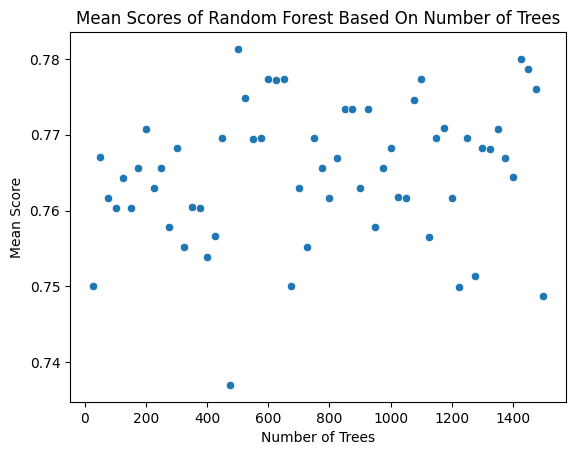
\includegraphics[width=1\linewidth]{mean_scores_num_trees.png}
    \caption{Graphing the mean score based on a number of trees ('Skin Thickness' and 'Insulin Level' features not used for model development)}
    \label{fig:enter-label}
\end{figure}

\begin{figure}
    \centering
    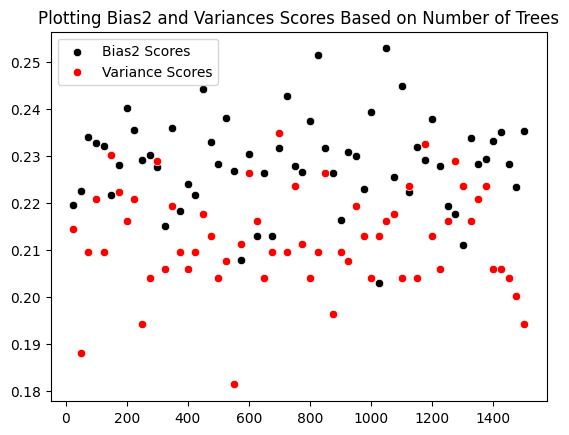
\includegraphics[width=1\linewidth]{bas2_variance_to.png}
    \caption{Attempt at Portraying a Bias-Variance Trade-Off}
    \label{fig:enter-label}
\end{figure}

\begin{figure}
    \centering
    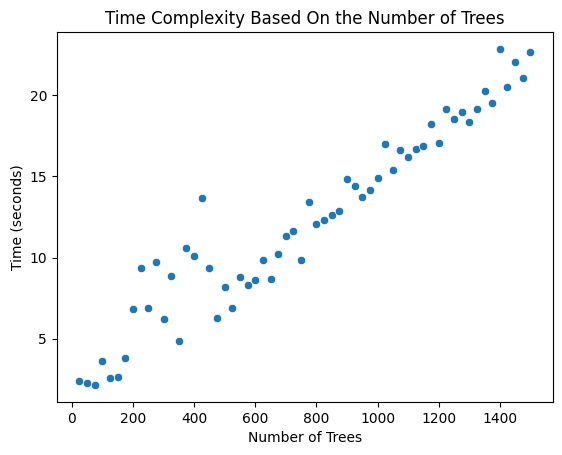
\includegraphics[width=1\linewidth]{time_complexity_nt_tuning.png}
    \caption{Time Complexity Based on the Number of Trees}
    \label{fig:enter-label}
\end{figure}

\section{Discussion}

Our model boasts an accuracy of 76.79\%, slightly higher than a previous study's 72\% accuracy with the same dataset and a Random Forest classifier (Mujumdar and V 2019). Still, there remains room for improvement.

For one, although we were able to identify outliers during EDA, we did not handle them. With additional time and research, we may elect to determine a method to remove these outliers with the hope of improving our model's performance.

Additionally, some issues lie within the dataset. The Pima dataset is highly specific, only including Pima women of a certain age range in Arizona. Therefore, the results of our model may not generalize to other populations, even one that is closely related, such as the Pima Indians of Mexico. With further research, we may wish to explore different T2D datasets with our chosen model.

Finally, we may also explore the performance of a greater variety of models, such as Logistic Regression, for a more thorough model selection process. As in Mujumdar and V's paper (2019), we may boost our model's performance with a new dataset, as well as pipelining the data for training to yield higher accuracies.

\section{Conclusion}

We propose a Random Forest Classifier for the task of predicting whether a patient has T2D. Our model is trained on the Pima dataset but with the features 'Skin Thickness' and 'Insulin' removed, as they were found to decrease the model accuracy when included. Our decision for this feature selection is further corroborated by an analysis completed using Random Forest, in which we determined that 'Skin Thickness' and 'Insulin' had the lowest feature contributions. Thus, we conclude that for our chosen model and dataset, these features are least relevant. However, different results may be produced with a different model and dataset. Further research is necessary to explore this possibility.

The link to the Github is as follows: \url{https://github.com/anniettr/t2d_pred}.

\appendices
\section{Project Roadmap}
In order to stay on track in completing our deliverables, we have separated our Development Plan into the following three milestones and deadlines:\\

\textbf{Milestone 1}: To be accomplished by May 15th
\begin{itemize}
    \item Reading relevant research papers including past work
    \item Understanding the dataset
    \item Exploratory Data Analysis (EDA)
\end{itemize}

\textbf{Milestone 2}: To be accomplished by May 26th
\begin{itemize}
    \item Developing an accurate prediction model
    \item Testing various parameters
    \item Evaluating the final model
\end{itemize}

\textbf{Milestone 3}: To be accomplished by June 8th
\begin{itemize}
    \item Building a basic front-end dashboard
    \item Recording the demo
    \item Finalizing the written report
\end{itemize}

\section{Assignment of Tasks}
\begin{itemize}
    \item Annie Tran
    \begin{itemize}
        \item Literature Review
        \item Feature Selection
        \item Discussion and Conclusion
    \end{itemize}
    \item Ivan Cvjetinovic
    \begin{itemize}
        \item Model Development and Selection
        \item Model Evaluation
        \item Dataset Splitting
    \end{itemize}
    \item Nikko Sanchez
    \begin{itemize}
        \item Dataset Trimming
        \item Imputation
        \item Model Deployment
    \end{itemize}
    \item Wanzhu Zheng
    \begin{itemize}
        \item Dataset Description
        \item Exploratory Data Analysis
        \item Random Sampling
    \end{itemize}
\end{itemize}

\section*{References}
Akmese, Omer F. 2022. Diagnosing Diabetes with Machine Learning Techniques. Hittite Journal of \textit{Science and Engineering,} 9(1) 9–18. https://doi.org/10.17350/HJSE19030000250\\

Chang, Victor, Jozeene Bailey, Qianwen Ariel Xu, and Zhili Sun. 2022. “Pima Indians Diabetes Mellitus Classification Based on Machine Learning (ML) Algorithms.” \textit{Neural Computing \& Applications} 35 (22): 16157–73. https://doi.org/10.1007/s00521-022-07049-z.\\

Dettori, Joseph R., Daniel C. Norvell, and Jens R. Chapman. 2018. “The Sin of Missing Data: Is All Forgiven by Way of Imputation?” \textit{Global Spine Journal} 8 (8): 892–94. https://doi.org/10.1177/2192568218811922.\\

IBM. n.d. “What Is the K-nearest Neighbors Algorithm?”\\

Mujumdar, Aishwarya, and V Vaidehi. 2019. “Diabetes Prediction Using Machine Learning Algorithms.” \textit{Procedia Computer Science} 165 (January): 292–99. https://doi.org/10.1016/j.procs.2020.01.047.\\
\

Schulz, Leslie O., and Lisa S. Chaudhari. 2015. “High-Risk Populations: The Pimas of Arizona and Mexico.” \textit{Current Obesity Reports} 4 (1): 92–98. https://doi.org/10.1007/s13679-014-0132-9.\\
\

Smith, Jack W., Everhart, J. E., Dickson, W. C., Knowler, W. C., and Johannes, R. S. 1988. "Using the ADAP Learning Algorithm to Forecast the Onset of Diabetes Mellitus." \textit{Proceedings of the} \textit{Annual Symposium on Computer Application in Medical Care,} 261–265.\\
\

“Type 2 Diabetes - Symptoms and Causes." 2023. Mayo Clinic. https://www.mayoclinic.org/diseases-conditions/type-2-diabetes/symptoms-causes/syc-20351193.\\


\ifCLASSOPTIONcaptionsoff
  \newpage

\fi


% that's all folks
\end{document}

